\lhead{\emph{Related work}}
\chapter{Related work}
% intro, current state on mobile music players
The rise of the smartphone and the introduction of music streaming services e.g. Spotify, Deezer, Pandora, WIMP and more have resulted in an increase in mobile music listening - in fact the number of mobile music listeners has more than doubled from 30 million active users in 2011 to over 70 million in 2013 according to a study in U.S. \cite{emarketer_music_2014}. Although mobile audio players have developed since the first portable cassette player by Sony in 1979 towards todays digital audio players with storage capacity e.g. smartphones, a similarity still remains - the way in which we interact with the device. E.g. like we needed the hands and eyes for rewinding or turning the tape on a cassette player, we need them as well for swiping to the preferred track in todays "typical" smartphone music application.

% typical interfaces, challenges
Todays "typical" music player user interface could cause interaction challenges when a user is on the move. Imagine a biking scenario where the user wants to change music track in a smartphone music application. This would require: Fetching the device e.g. from a pocket, switching the screen on, maybe unlocking the screen with a password, navigating through the music application GUI, switch the screen of, put smartphone back in pocket. Also the smartphone touch interface requires bare fingers for input recognition so removing gloves (in winter season) could also be a step in the process. A process that happens while the user is navigating through traffic. Studies show that while a user is doing an activity a vital factor is to minimize the amount of distraction for interaction modes \cite{pascoe_using_2000}.

Two research areas covers a great part of this kind of mobile interaction and they are presented in this chapter; Mobile HCI and Multimodal Interaction. Finally specific mobile systems that uses an alternative interaction form including mobile music players are presented in the last section. A graphical overview is shown in fig. \ref{fig:venn}.

\begin{figure}[htbp]
	\centering
		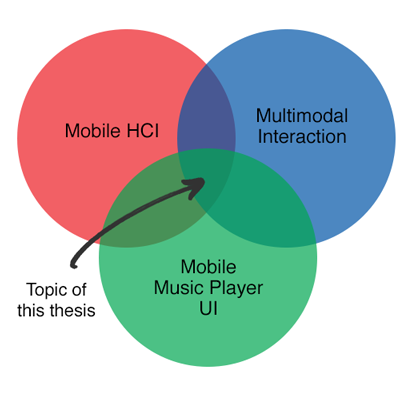
\includegraphics[width=0.5\textwidth,height=\textheight,keepaspectratio]{./Figures/venn.png}
		\rule{35em}{0.5pt}
	\caption[Venn diagram]{Thesis topic position}
	\label{fig:venn}
\end{figure}


\section{Mobile Human Computer Interaction}
The term "Human Computer Interaction" involves the study, planning and design of the interaction between human and computers \cite{card_psychology_1983}. This term supports a view both from the computer and from the human perspective. From a computer perspective in the mobile HCI community challenges like short battery life, network volatility, limited memory/processing power typically arise and specific system design patterns have been designed to handle this \cite{roth_patterns_2002}. From a mobile human perspective the term "nomadic computing" can be used where the main requirements for such a system is defined as providing capabilities and services to the nomad as he/she moves from place to place in a transparent, integrated and convenient way \cite{sawhney_nomadic_2000}.

% this project
In this project a mobile music player for cyclists is developed so the focus will be on the interaction between a user and device while the user is in motion. This kind of interaction has also been defined as "interaction in motion" \cite{marshall_mobile_2013}.

\subsection{Interaction in motion}
\label{sec:interactioninmotion}
According to Marshall and Tennent \cite{marshall_mobile_2013} mobile interaction does not exist as most mobile systems are designed for active interaction when a user is standing still dedicating his/her full attention to the device. Specific mobile systems should instead allow the user to interact while in motion e.g. driving, running or in this thesis case biking. To develop such kind of system specific challenges needs to be solved and Marshall and Tennent have classified these into four categories \cite{marshall_mobile_2013}:

\begin{description}
\item[Cognitive Load]
Cognitive Load Theory (CLT) has to do with managing a humans working memory (or short-term memory). It is also concerned with learning complex cognitive tasks. A learner can quickly become overwhelmed (the working memory is limited in capacity) by the number of information elements and their interactions that needs to be processed simultaneously. This can cause loss of information i.e. learning is not meaningful. On a higher level this could mean that a person is only able to pay attention to a certain amount of things at once. When the working memory limit is reached the person stops paying attention to other things. So even though a person is able physically to sense, hear or feel multiple interaction tasks, it may not be possible to attend to all these tasks at the same time. Controlling this cognitive high load has become the main focus of CLT \cite{paas_cognitive_2004}.

% Types of cognitive load
Paas et. al \cite{paas_cognitive_2004} distinguishes between three types of cognitive load; \textit{intrinsic}, \textit{extraneous} and \textit{germane}. The load is called intrinsic if it is imposed of the number of information elements and their interactivity. E.g. making a phone call while solving a puzzle contains two interactivities. If it is imposed by the manner in which the information is presented to the user or by the learning activities required of the user it is called extranous or germane. E.g. when making phone calls a discussion with an interviewer is less distracting than performing a simple memory test \cite{nunes_cognitive_2002}. The difference between extranous and germane load is expressed in their effectiveness meaning how the load is helpful in building schemas and automation so that the next time the user is presented with the same task, it becomes easier to implement i.e. the cognitive load is lower. Here the extranous load is in-effective while the germane load is effective.

% from the systems point of view
From a mobile interactive systems point of view the cognitive load could depend on environmental factors or the movement activity in which the user is performing e.g. walking a plane ground vs. climbing stairs (extranous/germane load). And if the person at the same time is forced to actively attend or respond to the system e.g. answering an important phone call, this would add another activity/interaction to the users working memory and possibly increase cognitive load (intrinsic load).

%can change over time. If a person is forced to actively attend or respond to the system the cognitive load is increased while a passive output from the system can decrease the cogntitive load.

% environment
%The cognitive load can also depend on environmental factors e.g. the movement activity in which the user is performing. Physical challenges e.g. walking a plane ground vs. climbing stairs can effect the mental demand of the user i.e. increase the cognitive load.

%It should be noted that the cognitive load research area is extensive. The theory described here is brief but sufficient for the focus of this thesis.

\item[Physical Constraints]
Mobile systems and user movement activities can both add constraints on the body position which could lead to a conflict making it hard or even impossible to interact. E.g. as mentioned earlier biking physically needs the hands for steering and eyes on the road while both of these body parts are used in the traditional smartphone interaction form (eyes on the screen, hands for touch gestures). This has been identified to be a major barrier to the use of mobile system whilst moving \cite{pielot_pocketmenu:_2012}.

\item[Terrain]
The terrain is described by the enviroment around a person while moving and interacting. Studies have shown that while running and interacting the terrain over which a person was running made a big difference in the interaction experience and the ability to concentrate on the output of the system \cite{marshall_using_2011}.

Physical terrain can be dynamic i.e. it can change over time while moving around different environments e.g. road obsticles, traffic, light level, rain, sound, etc. This could not only affect the user interaction experience but also the electronic device e.g. water or extreme cold/heat.

\item[Other people]
This class relates to other people during an interaction. For example in a crowded place the user needs to take care of people passing by while interacting with the mobile device. Or When biking the user needs to take care of people making an overhaul, communicating or waving back to a friend on the sidewalk. The social aspect of the environment a person is in can also have an impact on the device interaction e.g. in a quiet place a person would probably not use speech commands to interact with a device as this would be socially impolite.
\end{description}


\section{Multimodal interaction}
While the previous section was about planning and designing the interaction between humans and computers, this section describes how the actual information between a human and computer could be exchanged. 

\subsection{Modality definition and use}
Bolt was one of the first to define the term modality in a study where speech and gesture in combination was used as input to a system \cite{bolt_put-that-there:_1980}. Modalities has something to do with the mode of communication according to the human senses and input devices activated by humans \cite{jaimes_multimodal_2007,tzovaras_dimitrios_multimodal_2008}. The human senses are \textit{sight}, \textit{touch}, \textit{hearing}, \textit{smell} and \textit{taste}. Input modalities of many computer input devices can then be considered to correspond to these senses e.g. cameras (sight), haptic sensors (touch), microphones (hearing). While the term multimodal has been used in many different contexts and disciplines this thesis will focus on Tzovaras definition: \textit{"During interaction, the user produces input modalities to the system and the system produces output modalities to the user. A multimodal interactive system is a system that uses at least two different modalities for input and/or output. And a unimodal system is a system which uses the same single modality for input and output"} \cite{tzovaras_dimitrios_multimodal_2008}. The word input is defined by \cite{jaimes_multimodal_2007} to be of great importance as in practice most interactions take place using multiple modalities e.g. typing a keyboard (touch) while looking at the keys or screen (sight) to see whats being typed.

% modality combinations
Modalities can be used in combination with each other in different ways. In the "Put that there" system \cite{bolt_put-that-there:_1980} modalities are used in a complementary combination as the user can point the items on a large display and select or move them by vocal commands. In this case gestures and speech modalities are strengthening each other. In other cases modalities can act simultaneously giving different kind of information about the same feature e.g. visual and acoustic alarms in a building. Both these modality combinations have no unexpected implications in terms of the information that needs to be delivered. Either the information can only be gained in one way (complimentary approach) or the user can choose which way to gain the information (simultaneous approach). A case where modality combinations can have unexpected behaviour is when a modality is replaced with another to deliver the exact same information e.g. gaining an overview of a music collection would seem unnatural with voice commands compaired to a visual overview. This causes a non-linear effect and introduce more complexity to the interaction system.

\subsection{Multimodality in mobile systems}
As mentioned in \ref{sec:interactioninmotion} interacting with a device in motion introduces different challenges like environmental and human attention factors. This could imply that for some mobile situations certain multimodal interaction types would fit better than others. Much of the interfaces work especially in wearable computing tends to focus on visual headmounted displays \cite{barfield_fundamentals_2000} e.g. Google Project Glass. But not only does visual displays occupy the users visual attention, they can also be obtrusive and hard to use in bright daylight \cite{geelhoed_safety_2000}. Visual displays power consumption is must often also high i.e. they drain a mobile device battery and they are expensive.

% Eyes-free interfaces term
Several work on both audio \cite{kajastila_eyes-free_2013,bonner_no-look_2010,brewster_multimodaleyes-freeinteraction_2003,zhao_earpod:_2007,vazquez-alvarez_eyes-free_2011} and haptic \cite{pasquero_haptic_2011,pielot_tactile_2011} interfaces use the term eyes-free which refers to controlling the state of a system without visual attention. This kind of interaction has shown to be desirable in some mobile situations \cite{oakley_designing_2007,yi_exploring_2012} and even improve efficiency compaired to traditional visual displays \cite{zhao_earpod:_2007}. Eyes-free interfaces can keep the users visual attention on the road while driving \cite{sodnik_user_2008} or walking around in the city \cite{vazquez-alvarez_eyes-free_2011}. It should be taken into account though that just because information comes from a different modality that the one in use, it doesn't mean that the user is not distracted cognitively as described in \ref{sec:interactioninmotion}.

% Eyes-free modalities focus
Eyes-free interfaces are not limited to specific modalities. As mentioned in \ref{sec:alternativemusicuis} input modalities like speech, gesture and touch combined with audio or haptic feedback can "detach" the eyes from the interface. As this project focus is on a concrete mobile scenario i.e. biking - not only should the interface be eyes-free but also "hands-free" (as biking requires steering). To avoid the use of \textit{sight} and \textit{touch} human senses the proposed interface includes head gestures as input and audio as output.

\subsection{Head gestures as input modality}

% intro - alternative head tracking methods
There exists different kinds of approaches when it comes to controlling a system with head gestures. Using cameras it is possible to effectively track head movements via facial recognition \cite{morimoto_recognition_1996} and gaze tracking makes it possible to control an object by fixating the eyes on that object while moving the head \cite{vspakov_enhanced_2012}. Thus these techniques do not require any hardware sensors e.g. accelerometer and gyroscope but in return a camera placed in front of the user. Although this method has been conducted for mobile devices \cite{mardanbegi_eye-based_2012} the setup will still require the eyes in a combination with head gestures as an input modality.

Instead sensor based detection of head movements could be used e.g. accelerometer and gyroscope. Both Brewster et. al \cite{brewster_multimodaleyes-freeinteraction_2003} and Park et. al \cite{park_gaze-directed_2011} have evaluated systems using this kind of sensor based head gesture input. With these interfaces it is possible to detect not only the head rotation (gyroscope) [TODO: with respect to what?] but also the acceleration (accelerometer) when the head is moving. There exists advanced algorithms for recognizing motion gestures \cite{lu_head_2005, kratz_combining_2013, akl_accelerometer-based_2010}.

\subsection{Audio as output modality}
\label{sec:audiomodality}
Replacing visual with audio output has shown to have a positive effect when interacting in motion. Brewster showed, by compairing visual and audio feedback when pushing buttons on the same GUI, that it was difficult for users to devote all their visual attention to an interface while walking, running og driving and that the interaction workload decreased with audio feedback \cite{brewster_overcoming_2002}.

% Speech vs Non-speech audio
Audio output can in general be divided into two categories \cite{rocchesso_sounding_2003}:
\begin{description}
\item{1: \textit{Speech audio}}, can use a computer recorded human voice like in a guided audio tour for tourists.
\item{2: \textit{Non-speech audio}}, can be used for presenting more complex information e.g. music or other sounds.
\end{description}

Work has shown that non-speech audio is effective in improving the interaction in mobile environments \cite{pirhonen_gestural_2002, sawhney_nomadic_2000}. [TODO: needs a more detailed discussion]

[TODO: egocentric vs exocentric audio output]

When presenting the audio it's important to consider the attention which is required by the user while this can have a great impact on the cognitive load. Brewster et. al \cite{vazquez-alvarez_eyes-free_2011} presents two kinds of attention-tasks:

\begin{description}
\item{1: \textit{Selective-attention task}}, presenting multiple audio streams the user selectively choose which one to assign the attention e.g. listening to a voicemail while listening to a music track. This results in a lower cognitive load.

\item{2: \textit{Divided-attention task}}, in this case the user is forced to respond to each audio stream presented e.g. talking over the phone while interacting with a calendar using a audio menu. The attention gets divided and result in a higher cognitive load.
\end{description}

[TODO: needs to be explained in more detail. the need from the digital service probably sometimes constrain the choice of audio presentation. also the multimodal and task context of the user probably matters a lot]


\subsection{Spatial audio}
% intro - what is spatial audio, HRTF
Spatial audio or 3D audio allows a sound source to appear as if it is coming from anywhere in space around a listener \cite{begault_3dd_1994}. This can be achieved by using HRTF (Head Related Transfer Function). HRTF attempts to model the frequency modulations of a sound entering the human ear from a given direction and is implemented in many soundcards today. This is an attempt to present sound as we normally hear it in the real world.

% Advantages refs
Spatial audio has shown to be effective in several aspects. William W. Gaver, a pioneer in audio interfaces, has explored the intuitiveness of presenting complex information to users in the form of audio \cite{gaver_sonicfinder:_1989}. Similarly Graham explores the advantages in reaction time when using "auditory icons" \cite{graham_use_1999}. Gaver presents the use of spatial sound icons \cite{gaver_auditory_1986}. In doing so, he draws forward the unutilized potential of creating natural interaction (hearing sounds and navigating through them as we would normally do in the real world) through spatial audio.

% Multiple sound sources, cognitive load effect
Previous research has also shown that spatial audio is a successful technique for segregating multiple audio streams \cite{schmandt_audiostreamer:_1995, walker_spatial_2000}. Brewster et. al \cite{vazquez-alvarez_eyes-free_2011} shows in a study that when users must be able to direct their attention selectively to each individual audio stream representing a task (selective-attention task) - spatial audio had a great effect. In this case the cognitive load was kept low as described in \ref{sec:audiomodality}.

[TODO]
with multiple audio streams, spatial sound can increase cognitive load if used improperly \cite{vazquez-alvarez_eyes-free_2011}


\section{Mobile Audio User Interfaces}
This section describes the systems that are most related to this project. Alternative mobile music player user interfaces are presented first - alternative in the sense that the interaction form is different from the traditional way (touch input and visual output). Also other systems - not music related - are presented. These systems uses an interaction form that is close to the desired one in this project. Finally all systems properties are compaired and visualised in a table.

\subsection{Alternative music player interfaces}
\label{sec:alternativemusicuis}
There exists music player interfaces that attempts to use eyes-free interaction when listening to music on the go and they are presented in this section.

% headset controller
Headset music controllers are physical buttons attached to the wire between headset and device (see figure \ref{fig:nokia}). This controller typically includes play, stop, next track, previous track and volume buttons. Such a controller would require only one hand from the user to interact with a music application. This kind of interaction though assumes the user has created a playlist and knows in which order the tracks follows to navigate efficiently to the wanted track. Also this kind of menu is 1-dimensional in the sense that numbers have to be placed in a sequence missing the opportunity to go into a submenu e.g. an album of an artist. It should also be taken into account that although only using one hand for interaction this could still create challenges e.g. when steering or hitting the breakes while biking could require both hands on the steering.

\begin{figure}[htbp]
	\centering
		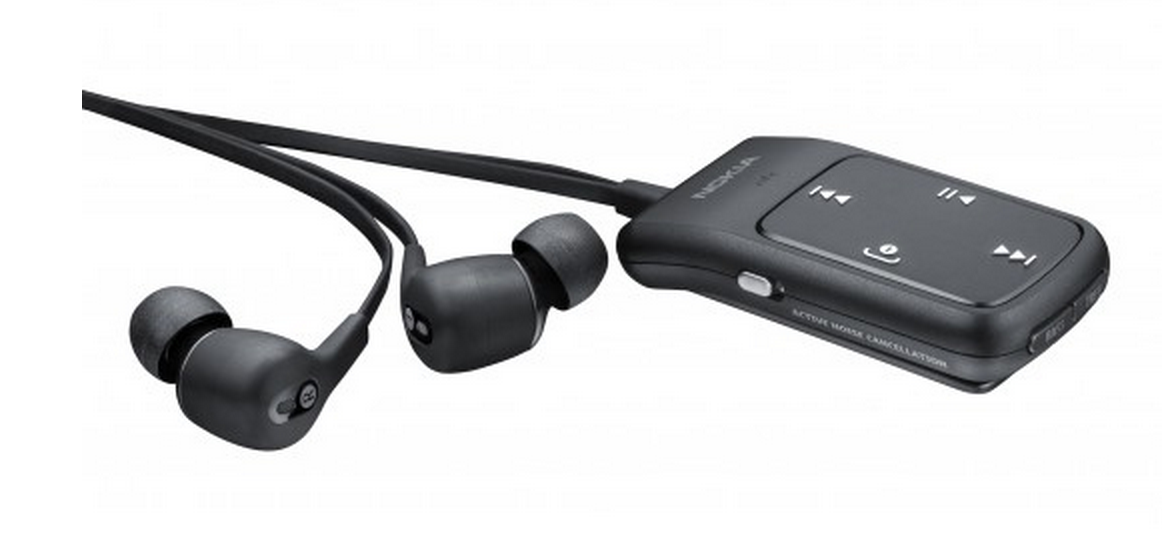
\includegraphics[width=0.6\textwidth,height=\textheight,keepaspectratio]{./Figures/nokia-headset.png}
		\rule{35em}{0.5pt}
	\caption[Nokia music headset]{A head music controller from Nokia \cite{nokia_launch:_2011}}
	\label{fig:nokia}
\end{figure}

% voice recognition
Voice recognition could also be used for navigating a music application \cite{stewart_boling_voice_2013}. In this application example the user could express simple commands like play, stop, next/previous track and queue. Voice recognition however introduces accuracy and stability challenges especially in mobile noisy environments. At the same time speech commands are limited - it would introduce even more complexity if the system should be able to interpret detailed commands e.g. an artist name or even a track title.

% other alternatives
Other more alternative music player interaction modes also exists using motion sensors. A system that use foot gestures for changing music track has been developed and shows a highly efficient way of interacting while running \cite{smus_running_2010}. Another system also using gesture recognition controls a music player by placing a device on different body parts e.g. placing it by side of the head while nodding changes the music track \cite{strachan_bodyspace_2007}. The systems are shown in figure \ref{fig:bodyandleg}.

\begin{figure}[htbp]
	\centering
		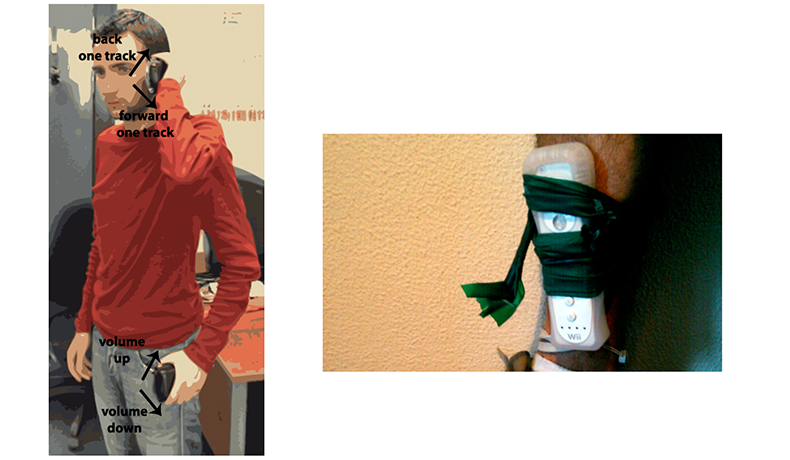
\includegraphics[width=0.8\textwidth,height=\textheight,keepaspectratio]{./Figures/bodyposeandleg.png}
		\rule{35em}{0.5pt}
	\caption[Alternative music players]{Figures from alternative music interfaces; Body Pose system \cite{strachan_bodyspace_2007} to the left and leg gesture system \cite{smus_running_2010} to the right}
	\label{fig:bodyandleg}
\end{figure}

All these systems have in common that they avoid the users visual attention but they are all limited to basic controls such as play, stop, next/previous track, volume up/down.

\subsection{Auditory gesture-based menus}
Other systems - though not all mobile music players - uses gesture based input modalities and audio as output modality and they can contribute to this projects final system in form of e.g. menu and audio design, navigation, etc.

% 1, Gestural and Audio Metaphors As a Means of Control for Mobile Devices
Pirhonen et. al \cite{pirhonen_gestural_2002} developed and evaluated a mobile music player that uses touch gestures and non-speech spatial audio to play/stop track, switch track and control volume. The device was an old pocket PC clipped to the users belt (device shown in figure \ref{fig:pirhonen}).

\begin{figure}[htbp]
	\centering
		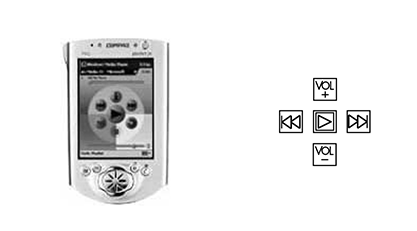
\includegraphics[width=0.6\textwidth,height=\textheight,keepaspectratio]{./Figures/pirhonen-system.png}
		\rule{35em}{0.5pt}
	\caption[Pirhonen system]{Figures from Pirhonen et. al \cite{pirhonen_gestural_2002} system showing the touch device (to the left) and touch menu (to the right)}
	\label{fig:pirhonen}
\end{figure}

The menu is designed so that swiping a finger in different directions on the touch screen results in an action e.g. changing track by swiping to the right. Spatial audio was used to play previous and next tracks respectively in the left (previous) and right (next) side in the users horizontal audio space while the current chosen track is playing in the center. Users perceived the menu through audio feedback as shown in figure \ref{fig:pirhonen} which almost matched the actual menu design.

An evaluation of the system showed significant usability improvements using gestures- and audio based interaction compaired to a visual pen-based interaction approach.


% 2, Interaction with eyes-free and gestural interfaces
Kajastila and Lokki \cite{kajastila_interaction_2013} also compaired auditory and visual menus but in this case they experimented with an input modality that was based on free-hand gestures. The free-hand gestures was detected by a camera and by moving the hand round in a circle the hand position mapped a sound item in the users spatial audio space i.e. a virtual circle around the users head. An illustration is shown in figure \ref{fig:kajastila}. The sound items were provided as speech-audio i.e. speech recorded numbers.

\begin{figure}[htbp]
	\centering
		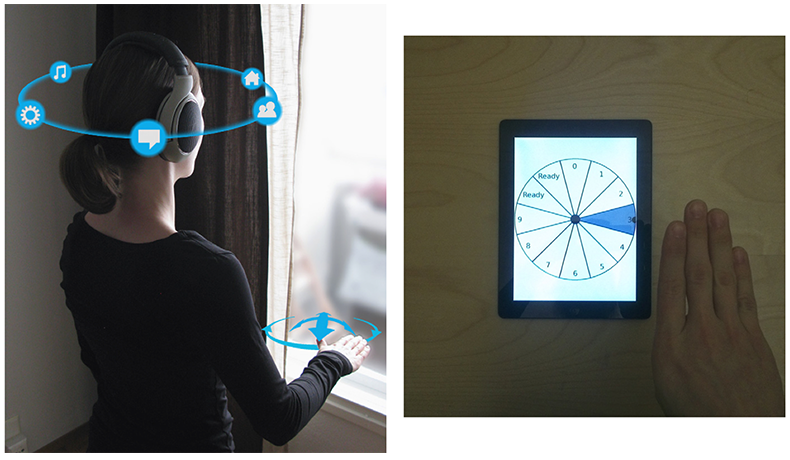
\includegraphics[width=0.8\textwidth,height=\textheight,keepaspectratio]{./Figures/kajastila-system.png}
		\rule{35em}{0.5pt}
	\caption[Pirhonen system]{Figures from Kajastila and Lokki \cite{kajastila_interaction_2013} system showing the free-hand navigation mapped to a users audio space}
	\label{fig:kajastila}
\end{figure}

The system was evaluated by users selecting specific numbers with free-hand gestures. The majority of the participants felt that an auditory circular menu was faster than a visual based menu.


% 3, Multimodal'eyes-free'interaction techniques for wearable devices
Brewster et. al \cite{brewster_multimodaleyes-freeinteraction_2003} developed and evaluated an eyes-free wearable system that uses head gestures as input modality and 3D audio as output modality. The systems hardware setup consists of headphones delivering 3D audio and a sensor attached for detecting the head orientation. These two hardware parts are connected via cables to a belt-mounted PDA running software that processes 3D audio and recognizes head gestures. The physical system is shown in figure \ref{fig:brewster}.

\begin{figure}[htbp]
	\centering
		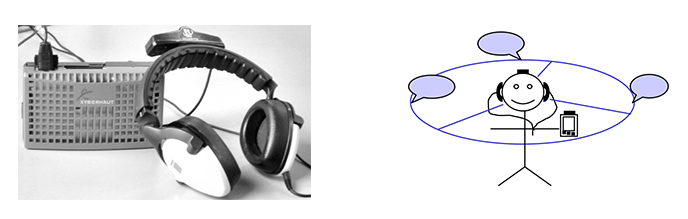
\includegraphics[width=0.9\textwidth,height=\textheight,keepaspectratio]{./Figures/brewster-system.png}
		\rule{35em}{0.5pt}
	\caption[Brewster system]{Figures from Brewster et. al \cite{brewster_multimodaleyes-freeinteraction_2003} system showing hardware setup (to the left) and interaction illustration (to the right)}
	\label{fig:brewster}
\end{figure}

The interaction design also illustrated in figure \ref{fig:brewster} consists of a 3D audio radial pie that uses head gestures for selecting items. More specifically audio sources are placed at positions in space around the user. The audio sources represents e.g. a phone-call, a news feed or stock market news and the user can then nod at a specific task to select it and drag it to the front of the audio space. Audio sources that the user finds less important can then be dragged to the rear of the audio space.

Evaluation of the system showed that sound and gesture can significantly improve the usability of a wearable device in particular under eyes-free mobile conditions and that head gestures was a successful interaction technique with egocentric sounds the most effective.


% 4, Gaze-Directed Hands-Free Interface for Mobile Interaction
Park et. al \cite{park_gaze-directed_2011} also experimented with head gesture input and audio output (though not spatial audio) but in this project focus was on the menu design. The hardware setup is custom build like the before mentioned system as a sensor is attached in this case to a cap for detecting head movement combined with headphones illustrated in figure \ref{fig:park}.

\begin{figure}[htbp]
	\centering
		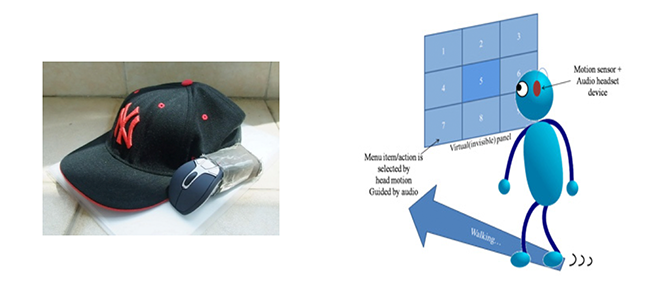
\includegraphics[width=0.9\textwidth,height=\textheight,keepaspectratio]{./Figures/park-system.png}
		\rule{35em}{0.5pt}
	\caption[Park system]{Figures from Park et. al \cite{park_gaze-directed_2011} system showing hardware setup (to the left) and interaction illustration (to the right)}
	\label{fig:park}
\end{figure}

The interaction design consists of different menus; a 1D horizontal/vertical, 2D grid and 2D circular menu and to navigate these menus different gesture models were tested as well. An illustration of this is showed in figure \ref{fig:park-menus}. As audio output the system uses speech audio to notify which item number is chosen.

\begin{figure}[htbp]
	\centering
		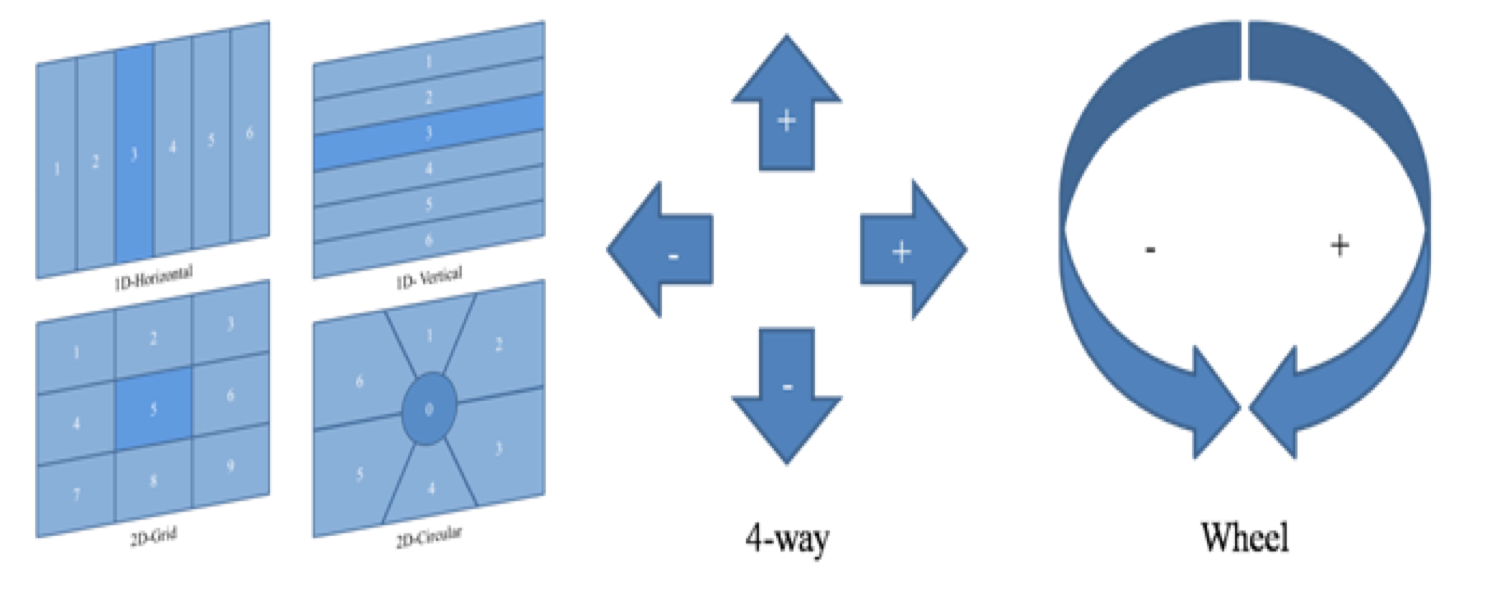
\includegraphics[width=0.9\textwidth,height=\textheight,keepaspectratio]{./Figures/park-menus.png}
		\rule{35em}{0.5pt}
	\caption[Park menus]{Figure from Park et. al \cite{park_gaze-directed_2011} system showing different menus (to the left) and gesture models (to the right)}
	\label{fig:park-menus}
\end{figure}

The system was tested with up to 12 number items and results showed that 2D grid menus was the most effective and had the lowest selection errors.


\subsection{Systems properties overview}
For this project specific properties of the system are required. Related systems that contains these properties can contain valuable input for this project. To give an overview and a better comparison - these properties are presented in table \ref{tab:related}.

\begin{table}[h] 
\caption{Related systems properties comparison} % title name of the table 
%\centering % centering table


\begin{tabular}{L{3cm}C{2cm}C{2cm}C{2cm}C{2cm}C{2cm}} \toprule
	Systems & In-motion interaction focus & Input modality & Output modality & Menu type and depth & Music application \\ \midrule
    %Properties & System 1 & System 2 & System 3 & System 4 \\ \midrule
    Voice recognition system \cite{stewart_boling_voice_2013}   & Yes & Speech input & Non-speech audio & 1D, simple commands & Yes \\
    \\
	Leg gesture system \cite{smus_running_2010}   & Yes & Leg gestures & Non-speech audio & 1D, simple commands & Yes \\ %\midrule
	\\
	Body pose system \cite{strachan_bodyspace_2007}   & No & Hand and head gestures in combination with device & Non-speech audio & 1D, simple commands & Yes \\
	\\
	Touch gesture system \cite{pirhonen_gestural_2002}   & Yes & Touch gestures & Non-speech audio, Spatial audio & 1D swipe direction based & Yes \\
	\\
	Free-hand gesture system \cite{kajastila_interaction_2013}   & No & Free-hand gestures & Speech audio, Spatial audio & Circular menu, 1D & No \\
	\\
	Head gesture system, Brewster et. al \cite{brewster_multimodaleyes-freeinteraction_2003}   & Yes & Head gestures & Non-speech and speech audio, Spatial audio & Circular menu, 1D & No  \\
	\\
	Head gesture system, Park et. al \cite{park_gaze-directed_2011}   & Yes & Head gestures & Speech audio, Spatial audio & Horizontal, vertical and grid menu, 2D & No \\
	\\
	This thesis system   & Yes & Head gestures & Non-speech (and simple speech) audio, Spatial audio & Circular menu, 2D & Yes, synced and evaluated against real world music application \\ \bottomrule
\end{tabular}

\label{tab:related} 
\end{table}








